\documentclass[border=.5mm]{standalone}
\usepackage[T1]{fontenc}
\usepackage{newtxtext}
\usepackage{tikz}
\usetikzlibrary{arrows.meta,backgrounds,calc}

\definecolor{promptnavy}{HTML}{1C3F60}
\definecolor{promptink}{HTML}{131820}
\definecolor{promptneutral}{HTML}{F2F2F4}
\definecolor{promptneutralstroke}{HTML}{B1B6BF}
\definecolor{promptrr}{HTML}{777777}
\definecolor{promptrrlight}{HTML}{EEEEEE}
\definecolor{promptsa}{HTML}{D55E00}
\definecolor{promptsalight}{HTML}{FAE8D9}
\definecolor{promptew}{HTML}{0072B2}
\definecolor{promptewlight}{HTML}{E1EEF6}
\newcommand{\revisionpromptfield}[1]{\textcolor{promptnavy}{\textit{\{#1\}}}}

\begin{document}
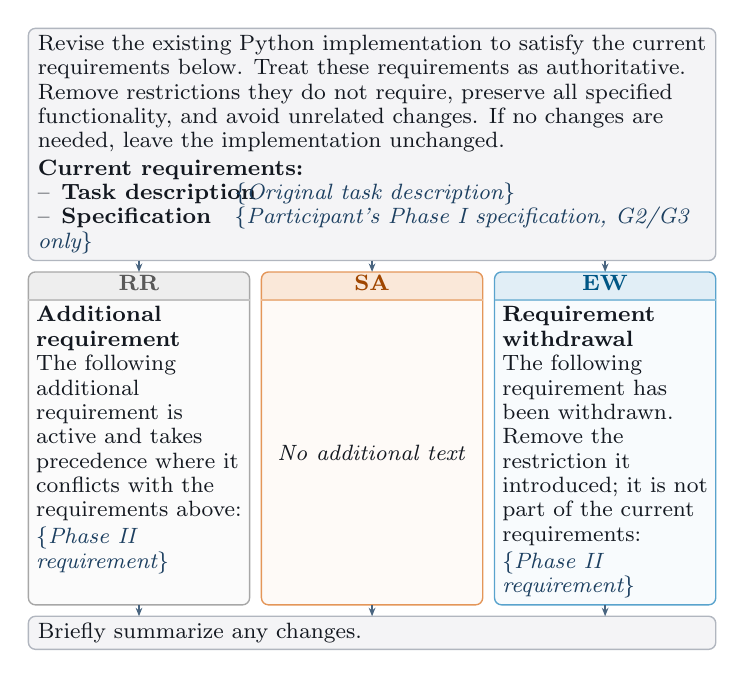
\begin{tikzpicture}[
    font=\fontsize{8}{8.8}\selectfont, text=promptink,
    prompt box/.style={anchor=north west, align=flush left, rounded corners=.9mm,
        line width=.5pt, outer sep=0pt, inner xsep=1.2mm, inner ysep=.85mm},
    prompt common/.style={prompt box, draw=promptneutralstroke, fill=promptneutral!85,
        text width=84.9mm},
    prompt condition/.style={prompt box, inner xsep=1mm, text width=26.1mm},
    prompt arrow/.style={draw=promptnavy!80, line width=.53pt,
        -{Stealth[length=1.08mm,width=.85mm]}},
]
    % The list punctuation formats the prompt's requirements fields for display.
    \node[prompt common] (opening) at (0,0) {%
        Revise the existing Python implementation to satisfy the current requirements below. Treat these requirements as \mbox{authoritative}. Remove restrictions they do not require, preserve all specified functionality, and avoid unrelated changes. If no changes are needed, leave the implementation unchanged.\\[1.1pt]
        \textbf{Current requirements:}\\
        \makebox[25mm][l]{\textendash\enspace\textbf{Task description}}\revisionpromptfield{Original task description}\\
        \makebox[25mm][l]{\textendash\enspace\textbf{Specification}}\revisionpromptfield{Participant's Phase I specification, G2/G3 only}
    };

    \coordinate (retained-top) at ([yshift=-1.45mm]opening.south west);
    \coordinate (alignment-top) at ([xshift=29.6mm]retained-top);
    \coordinate (withdrawal-top) at ([xshift=59.2mm]retained-top);
    \node[prompt condition] at ([yshift=-3.55mm]retained-top) {%
        \textbf{Additional requirement}\\
        The following additional requirement is active and takes precedence where it conflicts with the requirements above:\\[1pt]
        \revisionpromptfield{Phase II requirement}
    };
    \node[prompt condition] at ([yshift=-3.55mm]withdrawal-top) {%
        \textbf{Requirement withdrawal}\\
        The following requirement has been withdrawn. Remove the restriction it introduced; it is not part of the current requirements:\\[1pt]
        \revisionpromptfield{Phase II requirement}
    };

    \coordinate (branch-bottom) at (current bounding box.south -| opening.west);
    \node[prompt common] (closing) at ([yshift=-1.45mm]branch-bottom) {Briefly summarize any changes.};
    \foreach \arm/\abbr/\accent/\tint in {
        retained/RR/promptrr/promptrrlight,
        alignment/SA/promptsa/promptsalight,
        withdrawal/EW/promptew/promptewlight} {
        \coordinate (\arm-right) at ([xshift=28.1mm]\arm-top);
        \coordinate (\arm-bottom-right) at (branch-bottom -| \arm-right);
        \coordinate (\arm-title) at ([xshift=14.05mm,yshift=-1.775mm]\arm-top);
        \begin{scope}[on background layer]
            \begin{scope}
                \clip[rounded corners=.9mm] (\arm-top) rectangle (\arm-bottom-right);
                \fill[\tint!22] (\arm-top) rectangle (\arm-bottom-right);
                \fill[\tint] (\arm-top) rectangle ([yshift=-3.55mm]\arm-right);
            \end{scope}
            \draw[\accent!65, line width=.5pt, rounded corners=.9mm]
                (\arm-top) rectangle (\arm-bottom-right);
            \draw[\accent!45, line width=.48pt]
                ([yshift=-3.55mm]\arm-top) -- ([yshift=-3.55mm]\arm-right);
        \end{scope}
        \node[inner sep=0pt, text=\accent!75!black] at (\arm-title) {\strut\textbf{\abbr}};
        \draw[prompt arrow] (opening.south -| \arm-title) -- (\arm-top -| \arm-title);
        \draw[prompt arrow] (branch-bottom -| \arm-title) -- (closing.north -| \arm-title);
    }
    \node[inner sep=0pt] at ($(alignment-top -| alignment-title)!.5!(branch-bottom -| alignment-title)+(0,-1.775mm)$)
        {\textit{No additional text}};
\end{tikzpicture}
\end{document}
